\documentclass[10pt,letterpaper]{article}
\usepackage[latin1]{inputenc}
\usepackage{amsmath}
\usepackage{amsfonts}
\usepackage{amssymb}
\usepackage{graphicx}
\usepackage{hyperref}
\usepackage[table]{xcolor}
\usepackage{listings}

\lstset{language=Java, basicstyle= \ttfamily\small,  showstringspaces=false} 

\author{Andrew Rosen\\ Original David Matuszek}
\title{Rabbit Season}
\date{}

\begin{document}
	
	\maketitle
	
	
	\begin{abstract}
		This assignment serves as a review all the concepts we've learned so far.  
		It's a graphical program, so you can explore the basics of how GUI's work in Java.
		You will also start learning how to work with others, as this is a two person project.
	
	\end{abstract}
	
	\section{Premise}
		
	This assignment is different than the others, as I've given you a full working program, but you will need to improve it to get a grade.
	
	A \texttt{Fox} is hunting the \texttt{Rabbit} in a small field, represented by a 2D grid.
	The field has many spaces, some of which have bushes, which block the view of the fox and the rabbit.
	The goal of the fox is to end up on the same space of the rabbit, where he catches and eats it.
	The goal of the rabbit is to evade the fox for 100 turns.
	
	You play as the rabbit.
	
	\subsection{Setup}
	To get started, download the zip file, unzip it, and put all the java files into the same project.\footnote{You might surprised that after you create a new project, its as easy as copy-pasting or drop and dragging the files into the project.}
	Run \texttt{RabbitHunt.java} and you will get something like the image below.
	
	
	\begin{figure}[h!]
		\centering
		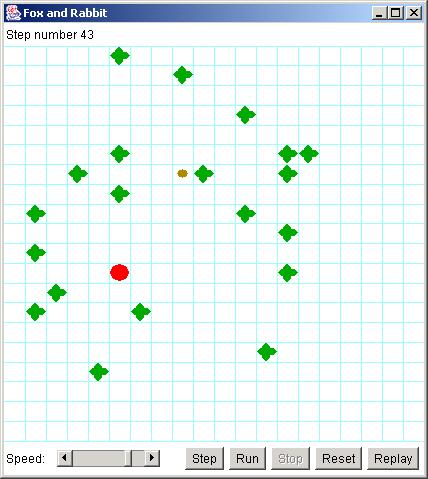
\includegraphics[width=0.7\linewidth]{hunt}
		\caption{The game board. If you get a window, but no grid, just hit one of the buttons in the window.}
		\label{fig:hunt}
	\end{figure}


	
	That big red dot is the fox, who is very hungry and is going to chase down and eat the rabbit (the brown dot).
	The green things are bushes.
	
	Play with the program for a while.
	Notice that the Fox always chases down the rabbit.
	This is because the Fox has a strategy, which you can look at in the \texttt{Fox.java} code.
	The Rabbit gets eaten all the time because its strategy is to just chooses a random direction to move.
	\newpage
	
	\subsection{Your Task}
	You need to fix that so that your Rabbit survives to turn 100 as much as possible.
	The \texttt{Rabbit} has a constructor \texttt{Rabbit(model, row, column)}, and it has a method \texttt{decideMove()}, which decides how the rabbit is going to move at each turn. 
	You can make as many changes to the Rabbit class that you want.
	
	Your grade is the percentage of times that the Rabbit makes it to turn 100 out of 300 runs (with some adjustment).
	It's probably impossible to get a 100.
	
	\subsection{The One Rule}
	You can only modify \texttt{Rabbit.java}.  
	You can look at everything else, but only change \texttt{Rabbit.java}.
	
	\newpage
	\section{Code Tour}
	This program is built using the Model-View-Controller paradigm.
	
	\begin{itemize}
		\item The \texttt{Model} holds the rules of the game and handles how the pieces interact with each other.\footnote{Technically, the Model is made of five classes: \texttt{Model}, all the animals, and \texttt{Bush}}
		The \texttt{Model} makes the board, places the \texttt{Fox}, the \texttt{Rabbit}, and a number of \texttt{Bush} objects.
		\item The \texttt{View} is the code for what you see.  \texttt{View}'s job is to show you, the user, what's going on in the \texttt{Model}.  
		In this program, that means \texttt{View} shows the game board.
		\item \texttt{Controller} lets you run the simulator.  It tells the \texttt{Model} when to start and stop.
	\end{itemize}
	
	Finally, \texttt{RabbitHunt.java} has the main method and just instansiates \texttt{Model}, \texttt{View}, and \texttt{Controller} objects, and turns control over to the \texttt{Controller} object.
	
	
	You can safely ignore and never open the \texttt{Controller} or \texttt{View} to complete this assignment.
	This means your code will use resources provided by \texttt{Model} and \texttt{Animal}.
	Those are the parts you need to get a good grasp of.
	
	\subsection{The Model}
	
	
	
	The Model class:
	\begin{itemize}
		\item places the fox, rabbit, and bushes in the field
			
		\item gives the rabbit and the fox each a chance to move (one moves, then the other--they don't both move at the same time)
		\item tells the \texttt{View} to display the result of these two moves, and
		\item determines which animal won
	\end{itemize}

	Model also provides you with many useful constants.
	Many aspects of the program, such as direction and what an animal can see are represented as an \texttt{int}.  
	Rather than remembering what number represents what, \texttt{Model} provides a number of constants.
	
	\begin{center}
	\begin{tabular}{ |l| l|}
		\hline
		\rowcolor{yellow}Model.N &	indicates "north" (straight up) \\\hline
		\rowcolor{yellow}Model.NE &	indicates "northeast" (up and to the right)\\\hline
		\rowcolor{yellow}Model.E &	indicates "east" (to the right)\\\hline
		\rowcolor{yellow}Model.SE &	indicates "southeast" (to the right and down)\\\hline
		\rowcolor{yellow}Model.S &	indicates "south" (straight down)\\\hline
		\rowcolor{yellow}Model.SW &	indicates "southwest" (to the left and down)\\\hline
		\rowcolor{yellow}Model.W &	indicates "west" (to the left)\\\hline
		\rowcolor{yellow}Model.NW &	indicates "northwest" (up and to the left)\\\hline
		\rowcolor{yellow}Model.STAY &	indicates "no move"\\\hline
		
		\rowcolor{green}Model.MIN\_DIRECTION &	the numerically smallest direction (not including STAY)\\\hline
		\rowcolor{green}Model.MAX\_DIRECTION &	the numerically largest direction (not including STAY)\\\hline
		\rowcolor[HTML]{AAACED} Model.BUSH &	indicates a bush\\\hline
		\rowcolor[HTML]{AAACED}Model.FOX &	indicates a fox\\\hline
		\rowcolor[HTML]{AAACED}Model.RABBIT &	indicates a rabbit\\\hline
		\rowcolor[HTML]{AAACED}Model.EDGE &	indicates the edge of the board\\\hline
	\end{tabular}
	\end{center}

	Finally, Model provides the following method:
	\begin{description}
	\item[\texttt{static int turn(int direction, int amount)}] Given a starting direction and the number of 1/8 turns to make clockwise, this method returns the resultant direction. 
	
	\end{description}
	
	For example, \texttt{turn(x,4)} would return the direction opposite of \texttt{x}.
	
	
	\subsubsection{The Other Model Classes}
	Other classes that form part of the Model are:
	\begin{description}
		\item[Bush] This class doesn't do anything. The Model creates bushes and places them, but the bushes themselves just sit there and get in the way.
		\item[Animal] This is the superclass for both the Rabbit class and the Fox class. It provides methods that are the same for both the rabbit and the fox: looking in a particular direction, measuring the distance to an object, and moving.
		\item[Fox] The fox is an animal that tries to catch and eat the rabbit.
		\item[Rabbit] The rabbit is an animal that tries not to get caught and eaten.
		
	\end{description}
	
	The Animal class provides the following methods. Since Fox and Rabbit are subclasses of Animal, they inherit these methods, and can use them just as if they had defined the methods themselves.
	\newpage
	\subsubsection{Animal Methods}
	\begin{description}
	\item[\texttt{int look(int direction)}]
	Return one of the constants Model.BUSH, Model.FOX, Model.RABBIT, or Model.EDGE, depending on what the animal sees in that direction.
	\item[\texttt{int distance(int direction)}]
	Returns the number of steps the animal would have to make in order to land on top of the nearest object (or go off the edge of the playing area).
	\item[\texttt{boolean canMove(int direction)}]
	Tells whether the animal can move in the given direction without being stopped by a bush or the edge of the board. Does not tell whether it's a good idea to move in that direction. 
	\end{description}
	
	
	
	\section{Hints}
	You should check out \texttt{Model.java} and  see what static resources it provides, as well \texttt{Animal.java}, as it provides all the common actions an \texttt{Animal} can do.
	
	If you're at a loss on where to begin, check out \texttt{Fox.java}, since it provides the algorithm for what the \texttt{Fox} does to chase down \texttt{Rabbit}.
	
	
	
	
	\section{Rubric}
	Most assignments are weighted at 100 points.
	This one will be weighted at 120.
	\begin{description}
		\item[100 points] The rabbit survival rate.  Your grade is the square root of the percentage of times the rabbit survives times ten.
		\item[20 points] You must explain your rabbit's survival strategy to me or the TA to get any credit at all for the assignment. 
		If you're nervous about describing your strategy in front of the Professor or your TA, I recommend commenting your code so you can read your comments like a script.
	\end{description}
	
	 
\end{document}